\section{Methodology}

\begin{figure}[htbp]
    \centering
    \begin{tikzpicture}[scale=0.5] % Adjust the scale factor as needed
      % Your TikZ code goes here
      \draw[fill=blue!30, line width = 1pt] (0,2) circle (1cm);
      \node at (0,2) {$n_{(0,0)}$};
      \node [text=red] at (-2,2) {1};
      \draw[fill=blue!30, line width = 1pt] (0,-2) circle (1cm);
      \node [text=red] at (-2,-2) {1};
      \node at (0,-2) {$n_{(1,0)}$};
      \draw[fill=orange!30, line width = 1pt] (5,4) circle (1cm);
      \node at (5,4) {$m_4$};
      \node [text=red] at (5,2.5) {1.5};
      \draw[fill=pink!30, line width = 1pt] (5,-4) circle (1cm);
      \node at (5,-4) {$n_{(3,1)}$};
      \node [text=red] at (5,-5.5) {1.5};
      \draw[fill=pink!30, line width = 1pt] (5,0) circle (1cm);
      \node at (5,0) {$n_{(2,1)}$};
      \node [text=red] at (5,-1.5) {1.9};
      \draw[fill=green!30, line width = 1pt] (10,0) circle (1cm);
      \node at (10,0) {$n_{(0,2)}$};
      \node [text=red] at (12,0) {$6.8$};
    \draw[->, >= angle 45, line width = 1pt, postaction={decorate, decoration={text along path, 
    text={0.55}, text align=center, raise=1mm}}](1, 2) -- (4, 4);
    \draw[->,>= angle 45, line width = 1pt] (1, -2) to (4, 4);
    \node at (3.75,3) {1};
    \draw[->,>= angle 45, line width = 1pt](1, 2) -- (4, 0);
    \node at (3.75,1) {0.95};
    \draw[->,>= angle 45, line width = 1pt](1, -2) -- (4, 0);
    \node at (3.75,-1) {0.55};
    \draw[->,>= angle 45, line width = 1pt](1, 2) -- (4, -4);
    \node at (3.75,-3) {1};
    \draw[->, >= angle 45, line width = 1pt, postaction={decorate, decoration={text along path, 
    text={0.5}, text align=center, raise=1mm}}](1, -2) -- (4, -4);
    \draw[-> , >= angle 45, line width = 1pt, postaction={decorate, decoration={text along path,
    text={1}, text align=center, raise=1mm}}] (6,-4) -- (9, 0);
    \draw[->, >= angle 45, line width = 1pt, postaction={decorate, decoration={text along path,
    text={1}, text align=center, raise=1mm}}] (6,0) -- (9, 0);
    \draw[->, >= angle 45, line width = 1pt, postaction={decorate, decoration={text along path,
    text={2}, text align=center, raise=1mm}}] (6,4) -- (9, 0);
   
    % \draw (1, -2) -- (4, 2);
    % \node at (3.75,1.25) {1};
  
    % \draw (1, 2) -- (4, -2);
    % \node at (3.75,-1.25) {1};
  
    % \draw[solid, postaction={decorate, decoration={text along path,
    % text={0.95}, text align=center, raise=1mm}}] (1, 2) -- (4, 2);
   


    % \draw[solid, postaction={decorate, decoration={text along path,
    % text={1}, text align=center, raise=1mm}}] (6,-2) -- (9, 0);
    % \draw[solid, postaction={decorate, decoration={text along path,
    % text={3}, text align=center, raise=1mm}}] (6, 2) -- (9, 0);

    \end{tikzpicture}
    \caption{Refining by our method: Culprit Neuron is 3 }
    \label{fig:tree_cut_refine}
  \end{figure}
  


\dmcmt{Im not leading with the lang of partial order here, instead defining a
    tree directly. This, I feel is easier to motivate and explain. What we have
    really is more than just a partial order of merge operations - it is in fact
    a tree. It is can be motivated by saying that it lets us define merge groups
    in a way that is in some sense optimal. It is also easier to explain
    precisely what the tree is by going over it's construction in an algo.
    The tree then can be used to define / talk about the partial order in the
intro, or the intro can itself be modified to refer to a tree instead. }

\todo{Add refs to later sections}
 
In this work we aim to utilize information from the semantic behavior of \cnc to
better control and guide the refinement process producing higher quality \abs
while retaining concrete soundness. 

In particular, we define a \textit{semantic
closeness factor} that captures how close the semantic-behavior of two 
neurons are. We utilise this semantic closeness factor to arrange the merge
operations into a tree where lower quality merges involving semantically far
neurons appear higher and can be refined with higher priority. 

Using this tree we build a framework \dmcmt{Is this okay?} where refinement can
be done by making cuts of this tree. We show that the merge groups coming from
such cuts have the property that any two neurons within the same group are 
semantically closer than any two neurons from two different groups. Thus, via
this tree-based refinement process, we are able to partition the neurons in \cnc
into merge groups\dmcmt{Is it clear what a merge group is?} in a manner that is
optimal with respect to the semantic information.
This allows us to avoid restoring large number of single neurons(see Section
\ref{s:nn-sam}) and lets us retain merge operations of higher quality. Thus, we
produce an \abs of the desired quality with a much smaller size. \todo{Ref later
sections}

While the choice of which nodes to leave merged together is guided by the cuts
of the tree, the weights attached to the abstract nodes are still chosen
by following the procedures from Section \ref{s:nn-sam} and \cite{cegar-nn}.
Thus, the concrete soundness guarantees still hold for the \abs obtained.

In the following sections we describe a general framework for such a unified
syntactic and semantic refinement process, describing each component in detail.
\linebreak

\dmcmt{This will be the general structure of the rest of this section. The
existing material can be re-organised into these headers.}

\subsection{Semantic Closeness Factor}

\dmcmt{ Talk about what the semantic closeness factor is. Say that it should
    characterise the semantic behavior, but doing so precisely is hard. So, talk
    about the simulation and observation vectors we use. Stress that this is a
    framework, and that one can explore other methods of semantic closeness
    within our framework. If we are able to get the characterestic based exps
    run, we can talk about that as well.
}

\subsection{Tree of Merges}

\dmcmt{ Talk about the tree of merge operations, maybe with example. Have
    explanation / algo about how tree is built, greedily choosing two best
    merges to do, like hcluster or existing Algo 2. Point out
    that worse merges are occurring higher. Don't talk about cuts or refinements
yet }


To establish the merging order of neurons, we create a tree 
structure wherein leaf nodes represent the original neurons, and 
non-leaf nodes represent merge groups. The construction of the tree 
follows a bottom-up approach, prioritizing the merging of similar neurons 
and delaying the merging of dissimilar ones. Similarity is ascertained through 
observation vectors.

In figure \ref{Figure: Order Of Merging}, if we give the list of input vectors $[[1], [2], [3]]$ to the observation function $o_{(i, j)}$ for $(n_{(1, 1, Inc)})$, then we obtain a list of output vectors $[[1.5], [3], [4.5]]$. We utilize the output of the observation function as a measure to merge neurons. For instance, considering three neurons $n_{(w, i)}$, $n_{(w, j)}$, and $n_{(w, k)}$ with 
observation vectors $o_{(w, i)}$, $o_{(w, j)}$, and 
$o_{(w, k)}$, the merging sequence adheres to the following conditions: 

If $||o_{(w, i)} - o_{(w, j)}||_{2} \leq ||o_{(w, i)} - 
o_{(w, k)}||_{2}$ and $||o_{(w, i)} - o_{(w, j)}||_2 \leq ||o_{(w, j)} - 
o_{(w, k)}||_{2}$, then $n_{(w, i)}$ and $n_{(w, j)}$ are initially merged into a 
representative neuron $\alpha$, followed by the merging of $\alpha$ and $n_{(w, k)}$. 
Here $||o_{(w, i)} - o_{(w, j)}||_{2}$ computes the ``$\textit{Euclidean 
Distance}$" between the observation vectors $o_{(w, i)}$ and  $o_{(w, j)}$.


In Figure \ref{Figure: Order Of Merging}, for the first layer, the initial 
merge would involve the neuron $n_{(1, 0, Inc)}$ with $n_{(1, 1, Inc)}$, 
forming $\textit{Merge 1}$, then we would combine $n_{(1, 2, Inc)}$ and 
$n_{(1, 3, Inc)}$, forming $\textit{Merge 2}$. Finally we combine 
$\textit{Merge 1}$ and $\textit{Merge 2}$ into the root node. 

As we progress up the tree, the degree of over-approximation rises. 
This is due to the increasing difference between observation vectors as 
we ascend. Therefore, the sub-trees closer to the root are indicative of 
coarser merges, whereas the ones farther from the root represent finer merges. 

\sncmt{Do we need to say how this tree corresponds to all possible merge groups
 which are allowed in the partial order because different cuts in the tree 
 correspond to different neural networks. If ``Yes'', do we need to include the 
 Guy Katz abstraction details. And then, in the next section, do we need to tell 
 how to construct the actual weight matrix from indexing into this all possible 
 merge groups weight matrix? Because Dig talked about efficient data structures 
 in the intro.}


\subsection{Tree-cuts and Refinement}
\label{s:refinement}



\begin{figure}[htbp]
    \centering
    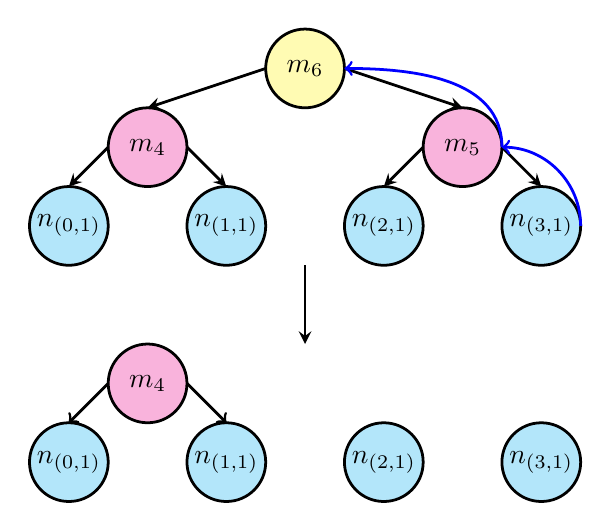
\begin{tikzpicture}[scale=0.5] % Adjust the scale factor as needed
        % Your TikZ code goes here
        \draw[line width=1pt,fill=yellow!30] (0,0) circle (1cm);
        \node at (0,0) {$m_6$};
        \draw[line width=1pt, fill=magenta!30] (-4,-2) circle (1cm);
        \node at (-4,-2) {$m_4$};
        \draw[line width=1pt, fill=magenta!30] (4,-2) circle (1cm);
        \node at (4,-2) {$m_5$};
        \draw[line width=1pt, fill=cyan!30] (-6,-4) circle (1cm);
        \node at (-6,-4) {$n_{(0,1)}$};
        \draw[line width=1pt, fill=cyan!30] (-2,-4) circle (1cm);
        \node at (-2,-4) {$n_{(1,1)}$};
        \draw[line width=1pt, fill=cyan!30] (6,-4) circle (1cm);
        \node at (6,-4) {$n_{(3,1)}$};
        \draw[line width=1pt, fill=cyan!30] (2,-4) circle (1cm);
        \node at (2,-4) {$n_{(2,1)}$};
        \draw[-> , >=stealth,line width=1pt] ({0 + cos(180)},{0 + sin(180)}) -- (-4,-1);
        \draw[->, >=stealth, line width=1pt] ({0 + cos(0)},{0 + sin(0)}) -- (4,-1);
        \draw[->, >=stealth, line width=1pt] ({-4 + cos(180)},{-2 + sin(180)}) -- (-6,-3);
        \draw[->, >=stealth, line width=1pt] ({-4 + cos(0)},{-2 + sin(0)}) -- (-2,-3);
        \draw[->, >=stealth, line width=1pt] ({4 + cos(180)},{-2 + sin(180)}) -- (2,-3);
        \draw[->, >=stealth, line width=1pt] ({4 + cos(0)},{-2 + sin(0)}) -- (6,-3);
        
        % Curved arrow
        \draw[->, color=blue, line width=1pt] (7, -4) to[out=90, in=0] (5, -2);
        \draw[->, color=blue, line width=1pt] (5, -2) to[out=90, in=0] (1, 0);
        \draw[->, >=stealth, line width=1pt] (0,-5) to (0,-7);

        \draw[line width=1pt, fill=magenta!30] (-4,-8) circle (1cm);
        \node at (-4,-8) {$m_4$};
        \draw[line width=1pt, fill=cyan!30] (-6,-10) circle (1cm);
        \node at (-6,-10) {$n_{(0,1)}$};
        \draw[line width=1pt, fill=cyan!30] (-2,-10) circle (1cm);
        \node at (-2,-10) {$n_{(1,1)}$};
        \draw[line width=1pt, fill=cyan!30] (6,-10) circle (1cm);
        \node at (6,-10) {$n_{(3,1)}$};
        \draw[line width=1pt, fill=cyan!30] (2,-10) circle (1cm);
        \node at (2,-10) {$n_{(2,1)}$};
    
        \draw[->, line width=1pt] ({-4 + cos(180)},{-8 + sin(180)}) -- (-6,-9);
        \draw[->, line width=1pt] ({-4 + cos(0)},{-8 + sin(0)}) -- (-2,-9);

    \end{tikzpicture}
    \caption{Trees and Cuts}
    \label{fig:Order_of_merging}
\end{figure}


\dmcmt{Connect cuts in tree to refinement, again with example. Describe the
    culprit based refinement process. Clarify that the culprit selection
heuristic can be replaced with any other heuristic within our framework.}

We are guided by this tree as a prospective refinement method. Starting with the 
entire tree where everything is merged. We leverage it to refine the network.
This process commences by identifying the ``culprit neuron $\gamma$'' 
selected for refinement. A ``culprit neuron'' in a merge group is selected 
on the basis of how much the neuron contributed to the output. If change in 
output of  neuron changes the value of the output neuron significantly then
that neuron is a good candidate for ``culprit neuron". 

Following this, we reverse all merges dependent on the culprit 
neuron $\gamma$. Therefore, refinement essentially involves finding a 
cut-point in the tree, precisely where all merges dependent on the 
culprit neuron $\gamma$ are undone. Each cut produces a set of trees, 
the merge groups then consist of neurons in the leaf nodes of the  these trees.
Therefore finding new merge groups for refinement is therefore just finding a 
cuts in the tree.

\sncmt{Do we need to tell the LCA algorithm here?}

Consider Figure \ref{Figure 2}, illustrating the merging sequence of 
neurons $n_{(1,0,Inc)}$, $n_{(1,1,Inc)}$, $n_{(1,2,Inc)}$, and 
$n_{(1, 3, Inc)}$. If, for instance, the neuron $n_{(1,3,Inc)}$ 
is identified as the problematic neuron based on a counter-example, 
we will reverse all the merges dependent on the $n_{(1,3,Inc)}$ neuron,
 including $\textit{Merge 2}$ and the $\textit{Root Node}$ merge. 
 Consequently, after implementing this reversal indicated in Figure 
 \ref{Figure 2}, our refinement phase will yield three distinct merge groups. 
 The first merge group comprises two neurons, namely $n_{(1,0,Inc)}$ and
 $n_{(1,1, Inc)}$. The second merge group and the third merge have single 
 neurons $n_{(1,2, Inc)}$ and $n_{(1,3,Inc)}$, respectively.

 A neuron, denoted as $\gamma$, is designated as a culprit neuron within a
specific layer when absolute value of the product of the difference between
$(v_{Rep(\gamma)}$ and $v_{\gamma})$ and the effective weight is maximized.
\todo{Add the 3 different methods generating counter-examples. Scores should be
avg over $\beta$ for a particular $\gamma$.}

$||(v_{Rep(\gamma)} - v_{\gamma})||_{2} \cdot |(\textit{effective\_weight})|$

In this context, $Rep$ signifies the representative neuron for neuron $\gamma$,
$v_{\gamma}$ represents the value of the neuron $\gamma$ at counter-example $\beta$
and $\textit{effective\_weight}$ represents the how much does the value of output
neuron changes with respect to change in the value of the neuron under consideration,
essentially corresponding to the ``$\textit{gradient}$'' at that particular example 
``$\beta$''.

\subsection{Optimality of Merge Groups}

\dmcmt{Briefly argue / prove why two neurons within same merge group is
    semantically closer than neurons across groups. Stress that this is good for
    quality of merges. Point out that this holds in the running example, and
contrast the quality and size with gk (if tracking example through gk). }




\begin{algorithm}
    \caption{Finding Cuts in the Tree (find\_new\_merge\_groups)}
    \begin{algorithmic}[1]
        \State $\gamma= \arg \max_i \|v_{Rep(i)} -v_i \|_2 \cdot | \textit{effective\_weight}| $ 
        \State Find a sequence of nodes, $t_1,t_2,t_3,..,t_k$ representing a  path from $t_1=$root to $t_k=\gamma$.
        \State Remove the nodes $t_1,t_2,..,t_{k-1}$ denoting the merges dependent on $\gamma$ through this path, leading to our connected tree being split into a collection of disconnected sub-trees.
        \State New merge groups are the leaf nodes in our disconnected graph.
    \end{algorithmic}
    \hspace*{\algorithmicindent} \textbf{Output} New Merge Groups
\end{algorithm}

% \subsection{Optimality of the Trees}
% Our objective is to determine the most efficient order for merging neurons, minimizing the introduction of over-approximation at each step. This approach aims to avoid creating networks with excessive over-approximation, which could lead to the generation of spurious counter-examples in response to queries. Opting not to mitigate over-approximation at each step would result in an increased number of refinement steps. This essentially entails making additional solver calls, incurring significant costs to eliminate the spurious counter-examples.


% Nevertheless, during the initial merging process (until saturation is reached), the root node ``$\rho$'' will exhibit the same level of over-approximation across all conceivable merging scenarios—for all possible tree sequences. Nevertheless, when we descend one level down the tree to explore the children nodes of our original root node $\rho$ for the purpose of identifying a cut for refinement, we discover varying levels of over-approximation manifesting in the root nodes of the resultant sub-trees. These differences are a result of the different merging scenarios pursued to construct those individual trees.

\begin{algorithm}[H]
\caption{Cluster Merging Algorithm (find\_abstraction\_tree)}
\label{Cluster Merging Algorithm}
\begin{algorithmic}[1]
    \State Initialize every simulated distance vector as a singleton cluster.
    \State Initialize $C=\{v_1,v_2,v_3,..\}$ as the set of singleton clusters.
    \State Initialize a Binary Tree $T$ with leaves as $\{(n_1),(n_2),(n_3),..\}$ corresponding to $\{v_1,v_2,v_3,..\}$.
    \State Initialize $V$ as a set of visited nodes, empty at first.
    
    \Function{MergeFunction}{$u, v$}
        \If{All nodes are classified as \textbf{Inc}}
        {
        
            \Return $\max(u, v)$
        }
        \Else{ }
        {
        
            \Return $\min(u, v)$
        }
        \EndIf
    \EndFunction
    
    \While{$|C|>1$}
        \State $v_j, v_j = \arg\min_{\substack{a, b \in C}} \| a - b \|_2$
        \State Set $w=\text{MergeFunction}(v_i,v_j)$
        \State Let nodes from $T$ not in $V$ corresponding to $v_i,v_j$ be $m_i$ and $m_j$
        \State Remove $v_i,v_j$ from $C$ and add $w$ to $C$.
        \State Make $(m_i \cup m_j)$ the parent of $(m_i)$ and $(m_j)$ in tree $T$
        \State Add $m_i$ and $m_j$ to $V$.
    \EndWhile
\end{algorithmic}
\end{algorithm}

% While the optimal tree, representing the optimal merging sequence, can aid in the refinement process by guiding the reversal of merges, finding such an optimal tree poses is extremely challenging. Even when dealing with only `n' Increment (Inc) neurons that have been merged to saturation, the total number of possible trees is given by $(2n-3)!!$, making the task of determining the truly optimal tree from these options extremely challenging.

% Since finding this ideal tree is a challenging task, we employ hierarchical clustering (Algorithm \ref{Cluster Merging Algorithm}) as an approach to approximate and derive such a tree. Initially, we simulate our network using a set of `$k$' inputs. Subsequently, we employ cluster analysis on these `$k$' points to construct a hierarchical arrangement of clusters. This process initiates with data points corresponding to simulated values (observation values in the observation vector) of a neuron  forming their own cluster. The clusters are then systematically combined based on their similarity, thereby generating a hierarchy of clusters. The choice of similarity measure is the ``$distance \hspace{1mm} metric$" between clusters. We have used ``$Euclidean \hspace{1mm} Distance$" as our distance metric. Given that the data points to perform this hierarchical clustering originate from the values of the simulated neurons, this hierarchical clustering effectively reflects the methodology we employ to merge the neurons.

% For example, in Figure \ref{Figure: Order Of Merging}, we conducted a simulation of our network on three data points. Subsequently, we examined the observation vectors corresponding to these points. Utilizing the hierarchical clustering algorithm, the initial selection for merging  will involve $(n_0^{1}, Inc)$ and $(n_1^{1}, Inc)$ because of the fact that their Euclidean distance is minimum. This forms $\textit{Merge 1}$ in Figure \ref{Figure: Order Of Merging}. The observation vector for $\textit{Merge 1}$ ($\nu_\textit{Merge1 }$) is the max of the $\nu((n_0^{1}, Inc))$ and $\nu((n_1^{1},Inc))$ which is \{1.5, 3, 4.5\}. For decrement nodes the observation vector would be minimum of the observation vector of the corresponding decrement nodes. The next merging step involved selecting $\nu((n_2^{1}, Inc))$ and $\nu((n_3^{1}, Inc))$ and merging these two neurons, representing $\textit{Merge 2}$ in Figure \ref{Figure: Order Of Merging}. The observation vector for $\textit{Merge 2}$ is now \{4, 8, 12\}. Ultimately, the Merge1 merge group is merged with the $\textit{Merge 2}$ merge group to create the Root Node in our network.

\begin{figure}[H]
    \centering
    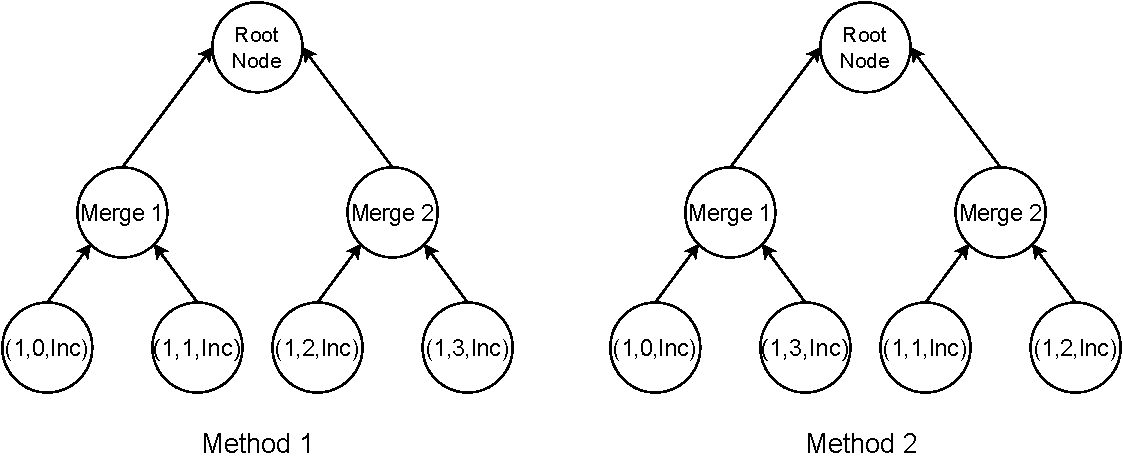
\includegraphics[width = 0.5\textwidth]{diagrams/good_vs_bad_merges.pdf}
    \caption{Ways of Merging}
    \label{Figure 3}
\end{figure}

% This approach of merging neurons based on similarity proves advantageous as it helps in reducing number of refinement steps. For instance, consider the task of checking whether $\forall v_{0}^{0} \in [0, 1]$ implies $v_{0}^{2} < 10$. If we had the neuron $(n_{3}^{1}, Inc)$ as the culprit neuron and then if we follow the second merging approach depicted in Figure \ref{Figure 3}, then we would have been compelled to reverse both $\textit{Merge 1}$ and $\textit{Merge 2}$. However, by employing the first merging approach, undoing only the $\textit{Merge 2}$ becomes sufficient, resulting in a reduction in the number of refinement steps required.


\subsection{Overall Algorithm}
\begin{algorithm}[H]
    \caption{Overall Algorithm}
    \label{Overall Algorithm}
    \begin{algorithmic}[1]
        \State $\mathcal{N'}$ = split\_Inc\_Dec($\mathcal{N}$)
        \State $\mathcal{N''}$ = abstract\_network($\mathcal{N'}$)
        \State simulation\_dict = simulate\_network($\mathcal{N'}$)
        \State $\mathcal{T}$ = find\_abstraction\_tree($\mathcal{N'}$, $simulation\_dict$)
        \If{verify($\mathcal{N''}$, $\kappa$, $\lambda$) is UNSAT}{

            \Return Property Holds
            }
        \Else
            \State Extract counter-example $\beta$
            \If{$\beta$ is not a spurious counter-example}
            {

                \Return ($\beta$, Property Violated)
            }
            \Else
                \State Find culprit neuron $\gamma$
                \State $merge\_groups$ = find\_new\_merge\_groups($\mathcal{T, \gamma}$)
                \State $\mathcal{N''} = get\_abstract\_network(merge\_groups)$
                \State \textbf{goto} step 5
            \EndIf
        \EndIf
    \end{algorithmic}
\end{algorithm}
